\documentclass[a4paper,11pt]{article}

\usepackage[english]{babel}
\usepackage[utf8x]{inputenc}
\usepackage{amsmath}
\usepackage{graphicx}
\usepackage{cite}
\usepackage{hyperref}
\usepackage{fullpage}
% \usepackage{apacite}
\setlength{\parskip}{1.2ex}
\begin{document}

\title{Open Information System: Conceptual schema}
\author{Thomas Perale -- 0546990\\Maximilien Romain -- 0543411\\Felipe Rojas -- 0542569\\Lehal Sherik -- 0543118}
\date{27 October 2017}

\maketitle

\section{Project subject}

The Webowl has eight classes, Category, Ebook, Purchase, Publisher, Author, User, Publisher, Role and Rating.
The User class has eight attributes which are pay information, name, email, password, userID, lastName, two roles "client" and "admin", which are further connected to the Role class.
The Purchase class has two attributes ID and Timestamp, and is bounded to User class by "isMaking" relation where the User is the domain and Purchase is the range. The Purchase class is also a master class to the "PaymentMethod" and "DeliveryMethod" classes.


The user class is also bounded to the eBook class, which has four attributes year, version, title and ISBN, by the relation "hasPurchased" and "manage" where the User is the domain and eBook class is the range. The ebook class is also a subclass of "ProductorService" class. The eBook class is related to Purchase class through the relation “isPartOf” where the domain is the ebook class and the range is the purchase class. 
The Rating class with two attributes ID and Number, is connected to eBook class with the domain eBook and range Rating and it is alos connected to the User class with the domain User and range Rating through the relations “hasRating” and “hasRated” respectively.

The eBook class is bounded to Category class, that has two attributes ID and description, by the relation "hasCategory". The domain here is ebook and the range is Category. The Category class also has the relation “subCategoryOf” which infers that an eBook can have two categories.

The eBook class is also bounded to the Publisher class by the relation "isPublishedby", where Ebook class is the domain and Publisher class is the range. The attributes of the Publisher class are the ID and name and it's also a subclass to "BusinessEntity" class.

The Author class, has three attributes, ID, first name and last name, and is bounded to Ebook class by "hasWritten" where the domain is the Author class and the range is the Ebook class. 

Rules

\section{Rules description}
First rule, If the book belongs to a category and that category is also a subcategory to another category, it implies that the book belongs to both the main category and it's subcategory. Example- If a book belongs to "war" category and the "war" category belongs to "action" category, it is implied that the book belongs to both "war" and "action" categories. This rule is relevant because an ebook can have more than one categories and some categories could be subcategories of one or more of these categories. The book has to belong to all the categories.\\
Ebook(?x), Category(?y), Category(?z), subCategoryOf(?y, ?z), hasCategory(?x, ?y), differentFrom(?y, ?z) $\rightarrow$ hasCategory(?x, ?z)

Second rule, If a user makes a purchase and an ebook is part of the purchase, then we can imply that the user “HasPurchased” an ebook. This rule is relevant to keep a track of purchased books. \\
User(?x), Purchase(?y), Ebook(?z), isMaking(?x, ?y), isPartOf(?z, ?y) $\rightarrow$ hasPurchased(?x, ?z)

Third rule, If a user has rated an ebook, it implies that the user purchased the ebook as the users can't rate a book without purchasing one. The rule is relevant because users who didn't purchase the book can't rate it. \\

User(?x), Rating(?y), Ebook(?z), hasRating(?x, ?y), hasRating(?z, ?y) $\rightarrow$ hasPurchased(?x, ?z)

The last rule implies that if a user has the role "admin", they can manage the ebooks database on the system. This rule is relevant because only the admin can manage the ebooks and not the normal users. \\
User(?admin), Ebook(?book), AdminRole(?role), hasAdminRole(?admin, ?role) $\rightarrow$ manage(?admin, ?book)

\section{ER Schema}

\begin{center}
  \makebox[\textwidth]{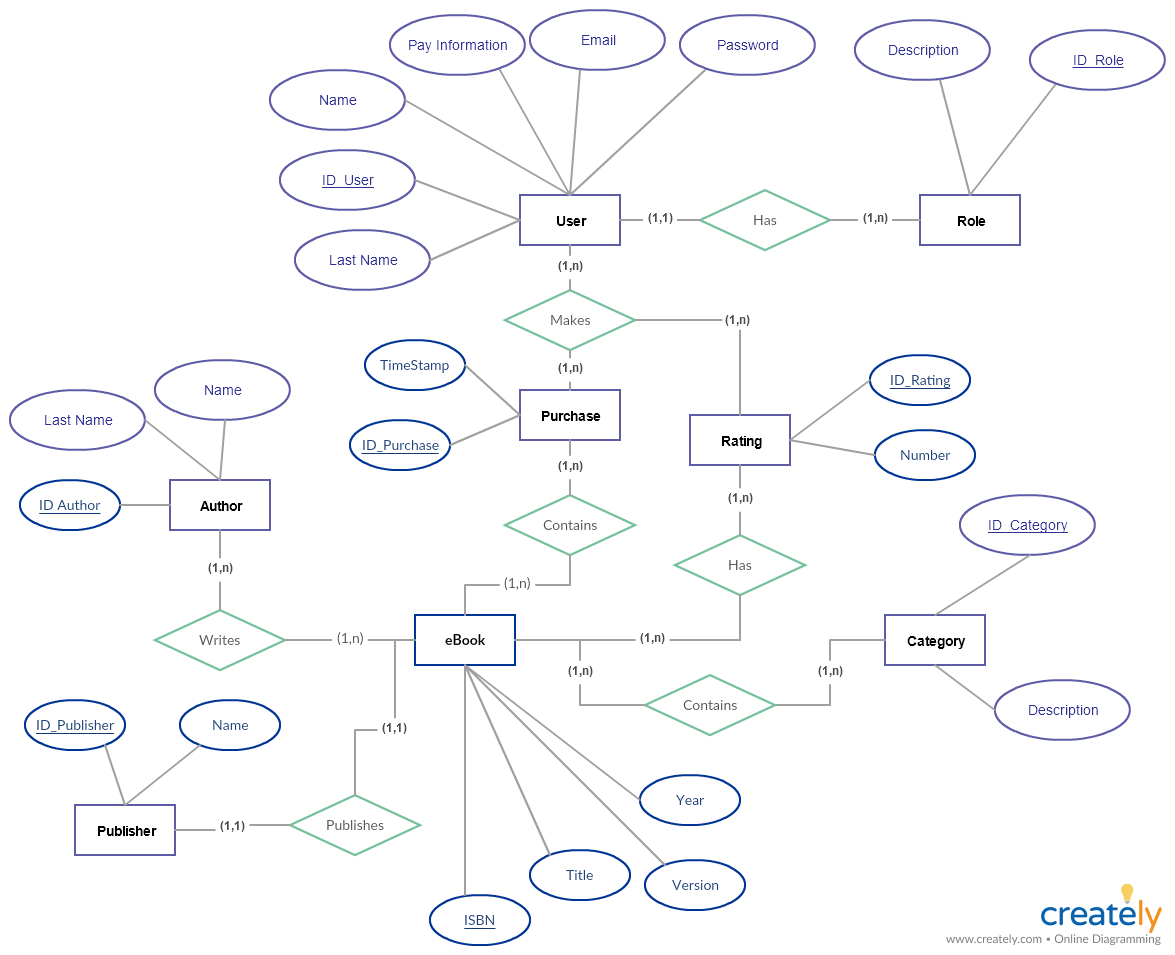
\includegraphics[width=\paperwidth]{ER_graph.png}}
\end{center}

\section{WebOwl visualisation}
\begin{center}
  \makebox[\textwidth]{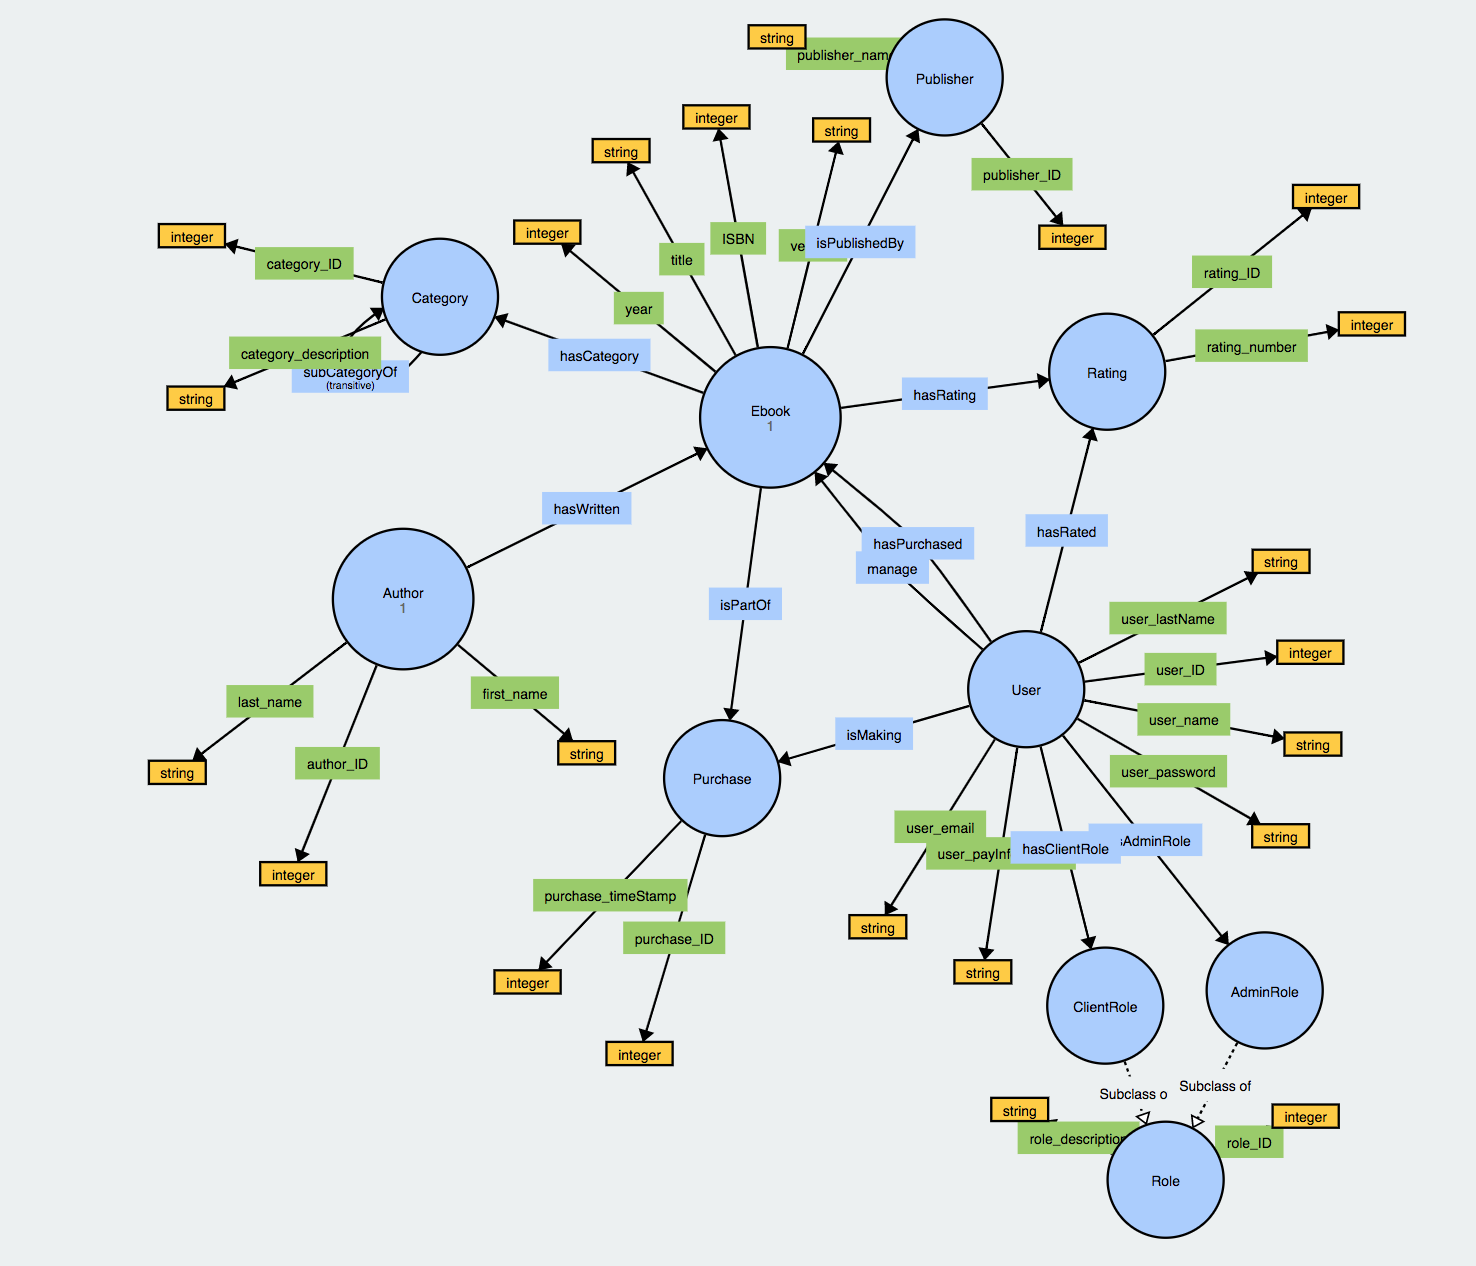
\includegraphics[width=\paperwidth]{webOwl.png}}
\end{center}


\end{document}
